% !TeX program = pdflatex
% !TeX encoding = UTF-8
%=======================================================================
%  GRIS-NOT-001  ·  Plantilla de notas rápidas para la memoria
%  Proyecto 00503 - Generator inspection robotic system · Mecanalisis
%  Identidad: GRIS-IDENTIDAD-001 v1.4
%-----------------------------------------------------------------------
%  CÓMO USARLA (en 3 pasos)
%
%   1. Copiá este archivo con el código de la nota, en su propia carpeta:
%         memoria/notas/02489-00-MC007/02489-00-MC007.tex
%      El número (###) es correlativo: mirá la última nota y sumá uno.
%      Las figuras van en memoria/notas/02489-00-MC007/figuras/ y el PDF
%      final se copia a memoria/pdf/.
%
%   2. Completá los cuatro datos del bloque «DATOS DE LA NOTA».
%
%   3. Escribí:
%        · Resultados (obligatorio, siempre primero): lo que se sabe
%          ahora que antes no se sabía. Frases cortas, con números.
%        · El resto es libre. Usá los títulos que te sirvan, o ninguno.
%
%   Compilar desde la carpeta de la nota:  pdflatex 02489-00-MC007.tex
%   En Overleaf: subí el .tex y logo-gris.pdf.
%
%  LOGO: se usa «logo-gris.pdf» (GRIS-LOGO-003, reducido) de esta carpeta
%  o de ../../plantilla/. Si falta, se escribe «GRIS» como marcador.
%=======================================================================
\documentclass[11pt,a4paper]{article}

%=======================================================================
%  DATOS DE LA NOTA  ← lo único que hay que tocar arriba
%=======================================================================
\newcommand{\codigo}{02489-00-MC009}          % 02489-00-MC###
\newcommand{\titulo}{Geometría de ranuras estatóricas}
\newcommand{\autor}{Matías Gaviño}
\newcommand{\fecha}{30/09/2026}                    % o p. ej. {24/09/2026}

%=======================================================================
%  ESTILO  (no hace falta tocar nada de aquí hasta \begin{document})
%=======================================================================
\usepackage[T1]{fontenc}
\usepackage[utf8]{inputenc}
\usepackage[spanish,es-noshorthands,es-tabla]{babel}
\usepackage{lmodern}
\usepackage[a4paper,top=3.0cm,bottom=2.4cm,left=2.4cm,right=2.4cm,
            headheight=20pt,headsep=1.2cm,footskip=1.1cm]{geometry}
\usepackage{microtype}
\usepackage{xcolor}
\usepackage{graphicx}
\usepackage{booktabs}
\usepackage{array}
\usepackage{enumitem}
\usepackage{titlesec}
\usepackage{fancyhdr}
\usepackage{caption}
\usepackage{amsmath,amssymb}
\usepackage{float}
\usepackage{tikz}
\usepackage[hidelinks]{hyperref}
\setlength{\emergencystretch}{3em}

% --- colores -----------------------------------------------------------
\definecolor{gris-naranja}{HTML}{FF7A00}   % naranja institucional
\definecolor{tinta}{HTML}{1E2328}
\definecolor{gris-medio}{HTML}{6B7280}
\definecolor{gris-linea}{HTML}{DADDE1}
\color{tinta}

\hypersetup{pdftitle={\codigo\ -- \titulo}, pdfauthor={\autor},
            colorlinks=true, linkcolor=tinta, urlcolor=tinta}

% --- logo ---------------------------------------------------------------
\graphicspath{{./}{figuras/}{../../plantilla/}}
\newcommand{\logogris}{%
  \IfFileExists{logo-gris.pdf}
    {
\includegraphics[height=16pt]{logo-gris.pdf}}
    {\IfFileExists{../../plantilla/logo-gris.pdf}
      {
\includegraphics[height=16pt]{../../plantilla/logo-gris.pdf}}
      {{\fontsize{18}{18}\selectfont\bfseries\sffamily\color{gris-naranja}GRIS}}}}

% --- tipografía del cliente (código documental) --------------------------
% Geogrotesque no es libre; se usa Roboto Condensed Bold, que viene con
% TeX Live y Overleaf y tiene el mismo aire que el logo.
\newcommand{\fuentecliente}{\fontfamily{Roboto-TLF}\fontseries{bc}\selectfont}

% --- encabezado y pie ---------------------------------------------------
\pagestyle{fancy}
\fancyhf{}
\renewcommand{\headrulewidth}{0.4pt}
\renewcommand{\headrule}{\vspace{3pt}{\color{gris-linea}\hrule height \headrulewidth}}
\fancyhead[L]{\logogris}
\fancyhead[R]{{\fuentecliente\fontsize{12}{12}\selectfont\color{gris-medio}\codigo}}
\fancyfoot[R]{\footnotesize\color{gris-medio}\thepage}

% --- títulos numerados ----------------------------------------------------
\setcounter{secnumdepth}{2}
\titleformat{\section}{\large\bfseries}{\thesection}{0.8em}{}
\titleformat{\subsection}{\normalsize\bfseries}{\thesubsection}{0.8em}{}
\titlespacing*{\section}{0pt}{16pt}{5pt}
\titlespacing*{\subsection}{0pt}{11pt}{3pt}

% --- texto ------------------------------------------------------------------
\setlength{\parindent}{0pt}
\setlength{\parskip}{6pt}
\linespread{1.05}
\setlist{topsep=2pt, itemsep=2pt, parsep=0pt, leftmargin=1.2em}
\setlist[itemize]{label={\raisebox{0.15ex}{\small$\bullet$}}}
\captionsetup{font={small,color=gris-medio}, labelfont=bf, skip=5pt}
\renewcommand{\arraystretch}{1.25}

% --- cabecera de la nota ------------------------------------------------------
\newcommand{\cabecera}{%
  \thispagestyle{fancy}%
  {\fontsize{20}{24}\selectfont\bfseries\titulo\par}%
  \vspace{5pt}%
  {\small\color{gris-medio}\fecha\quad·\quad\autor\par}%
  \vspace{6pt}}

% --- ayudas opcionales --------------------------------------------------------
% \figura{archivo}{ancho}{pie}
\newcommand{\figura}[3]{%
  \begin{figure}[htbp]\centering
    \includegraphics[width=#2\linewidth]{#1}\caption{#3}
  \end{figure}}

%=======================================================================
\begin{document}
\cabecera

\section{Resultados}

Solo máquinas reales de 20~MW o más. Los rangos son el mínimo y el máximo de lo
publicado, sin extrapolar. «Leída» quiere decir que se abrió la fuente primaria y
el número está en ella. «No abierta» quiere decir que la fuente existe pero no se
pudo abrir (ResearchGate, IEEE o Scribd). En ese caso el dato viene del material de
partida y no está verificado.

\begin{table}[H]\centering\small
\caption{Rangos comprobados en máquinas reales. Entre paréntesis, la cantidad de datos.}
\label{tab:resumen}
\begin{tabular}{l c c c c}
\toprule
 & \multicolumn{2}{c}{Hidrogeneradores} & \multicolumn{2}{c}{Turbogeneradores} \\
\cmidrule(lr){2-3}\cmidrule(lr){4-5}
Magnitud & Leída & + no abierta & Leída & + no abierta \\
\midrule
Ancho de ranura $b_s$ [mm] & 23,2 -- 28,0 (4) & 23,2 -- 30,0 (7) & 70 (1)$^{*}$ & 70 (1)$^{*}$ \\
Paso $\tau_s$ [mm] & 63,2 -- 67,9 (3) & 63,2 -- 99,7 (6) & 98,4 -- 128,4 (2) & 98,4 -- 128,4 (2) \\
$b_s/\tau_s$ [\%] & 38,8 -- 41,9 (2) & 35,1 -- 41,9 (3) & 71,1 (1)$^{*}$ & 71,1 (1)$^{*}$ \\
Ranuras $Q_s$ & 162 -- 810 (6) & 162 -- 810 (10) & 36 -- 42 (2) & 36 -- 60 (3) \\
Profundidad $h_s$ [mm] & 159,5 (1) & 159 -- 210 (3) & 160 (2) & 160 (2) \\
\bottomrule
\multicolumn{5}{l}{\footnotesize $^{*}$ Un solo dato, interpretado: la fuente dice «160$\times$70» sin decir cuál es el ancho.}
\end{tabular}
\end{table}

\begin{itemize}
  \item \textbf{Ancho de ranura en hidro: 23,2 a 28,0~mm comprobado} en cuatro
    máquinas de 34~MW a 145~MW. Con las fuentes no abiertas llega a
    \textbf{30~mm} (Gezhouba, 150~MW). No apareció ninguna ranura hidro más ancha.
  \item \textbf{Ancho de ranura en turbo: un solo dato, 70~mm}
    (QFSN-600-2YHG, 667~MVA). Sale de un modelo de elementos finitos que da
    «160$\times$70» sin rotular. No hay ningún otro turbo real con ancho
    publicado en la búsqueda. \textbf{El rango turbo no está comprobado.}
  \item \textbf{$b_s/\tau_s$ en hidro: 38,8 a 41,9\,\%} con fuente leída, y
    \textbf{35,1 a 41,9\,\%} sumando Manic-2. El 19,5\,\% que daba el
    material de partida (CB 870/300-28) \textbf{no es confiable}: sale de un
    diámetro interior de 15,8~m que no es coherente con la designación de la
    máquina (870~cm de diámetro exterior) ni con su velocidad periférica
    (177~m/s). Con 7,91~m da 39,1\,\%, dentro del rango anterior (§\ref{sec:cb}).
  \item \textbf{Paso de ranura: hidro 63 a 68~mm comprobado} (hasta
    \textbf{100~mm} en Itaipú, no abierta). \textbf{Turbo: 98 a 128~mm}, en dos
    máquinas de 600 y 1000~MW.
  \item \textbf{Cantidad de ranuras: hidro 162 a 810, turbo 36 a 42} (60 con
    la fuente no abierta). La diferencia viene de los polos:
    $Q_s = 3\,P\,q$, con 14 a 84 polos en hidro y 2 en turbo.
  \item \textbf{Todas las ranuras relevadas miden entre 159 y 210~mm de
    profundidad}, en hidro y en turbo.
  \item \textbf{Se descartan las envolventes del material de partida}
    ($b_s \le 75$~mm en hidro, $b_s \le 120$~mm en turbo, $b_s/\tau_s$ de
    12 a 75\,\%). Son extrapolaciones, no máquinas. También se sacan del rango
    los tres diseños de 250~MW de Minko y el modelo de 30~MVA: no son máquinas
    instaladas (§\ref{sec:disenos}).
  \item \textbf{No se encontró norma que fije $b_s/\tau_s$.} La geometría de
    ranura la define cada fabricante.
  \item \textbf{Pendiente:} incorporar las máquinas relevadas por Mecanalisis
    (turbos y otras, en la carpeta «001\_Estatores de referencia»), que no se
    pudieron leer desde esta sesión. Son lo que puede cerrar el rango turbo.
    Conseguir los textos no abiertos (Manic-2, CB 870/300-28, Gezhouba).
\end{itemize}

\figura{bs-vs-paso.pdf}{0.72}{Ancho de ranura contra paso en el diámetro
interior, para las máquinas reales con los dos datos. Las rectas grises son
$b_s/\tau_s$ constante. Los círculos vacíos son fuentes no abiertas. El CB
870/300-28 aparece con sus dos diámetros posibles.}

\section{Criterio y definiciones}

\subsection{Pregunta y criterio de evidencia}
El robot tiene que andar sobre el diámetro interior del estator o sensarlo. Hace
falta saber qué ancho de ranura, qué paso y qué relación entre los dos aparecen
en generadores de 20~MW o más. La nota parte de un informe preliminar hecho con
ChatGPT (\texttt{fuentes/material\_de\_partida.md}). Se revisó cada número contra
su fuente y se dejó fuera todo lo que no sea una máquina real.

Cada máquina tiene un nivel:
\begin{itemize}
  \item \textbf{A, leída:} máquina real o tipo real; la fuente primaria se abrió
    y el número está ahí. Las páginas usadas quedaron en \texttt{fuentes/}.
  \item \textbf{B, no abierta:} máquina real, pero la fuente no se pudo abrir.
    El dato es del material de partida. Si un buscador confirmó parte de él, se
    aclara.
  \item \textbf{D, diseño:} diseño propuesto o modelo teórico. Se lista pero
    no entra en ningún rango.
\end{itemize}

\subsection{Magnitudes}
\begin{itemize}
  \item \textbf{Paso de ranura} en el diámetro interior $D_i$, con $Q_s$ ranuras:
    $\tau_s = \pi D_i / Q_s$.
  \item \textbf{Ancho de ranura} $b_s$: el ancho del cuerpo de la ranura, que es
    el que publican las fuentes («slot width»). Ninguna fuente da la boca de
    ranura $b_{so}$ ni el ancho visible de la cuña.
  \item \textbf{Relación} $k_s = b_s/\tau_s$ y \textbf{diente en el diámetro
    interior} $b_t = \tau_s - b_s$. Suponen ranura de lados paralelos, sin
    labios en la boca.
  \item \textbf{Ranuras por polo y fase} $q = Q_s/(3P)$, con $P$ polos. Puede ser
    fraccionario.
\end{itemize}

\begin{figure}[H]\centering
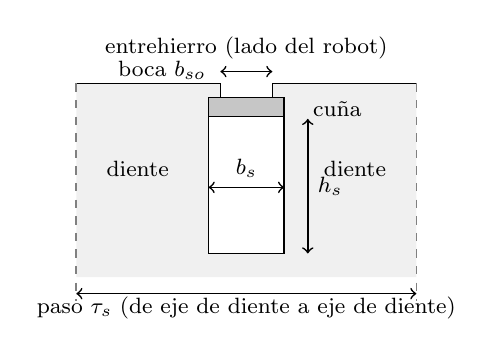
\begin{tikzpicture}[scale=0.6, line width=0.6pt]
  \fill[gray!12] (-3.6,0) -- (-0.55,0) -- (-0.55,-0.3) -- (-0.8,-0.3) -- (-0.8,-3.6)
        -- (0.8,-3.6) -- (0.8,-0.3) -- (0.55,-0.3) -- (0.55,0) -- (3.6,0) -- (3.6,-4.1) -- (-3.6,-4.1) -- cycle;
  \draw (-3.6,0) -- (-0.55,0) -- (-0.55,-0.3) -- (-0.8,-0.3) -- (-0.8,-3.6)
        -- (0.8,-3.6) -- (0.8,-0.3) -- (0.55,-0.3) -- (0.55,0) -- (3.6,0);
  \filldraw[fill=gray!45] (-0.8,-0.3) rectangle (0.8,-0.7);
  \node[font=\footnotesize, right] at (1.2,-0.55) {cuña};
  \node[font=\footnotesize] at (0,0.75) {entrehierro (lado del robot)};
  \draw[<->] (-0.55,0.25) -- (0.55,0.25);
  \node[font=\footnotesize, left] at (-0.65,0.28) {boca $b_{so}$};
  \draw[<->] (-0.8,-2.2) -- (0.8,-2.2) node[midway, above, font=\footnotesize] {$b_s$};
  \draw[<->] (-3.6,-4.45) -- (3.6,-4.45);
  \node[font=\footnotesize] at (0,-4.75) {paso $\tau_s$ (de eje de diente a eje de diente)};
  \node[font=\footnotesize] at (-2.3,-1.8) {diente};
  \node[font=\footnotesize] at (2.3,-1.8) {diente};
  \draw[<->] (1.3,-0.75) -- (1.3,-3.6) node[midway, right, font=\footnotesize] {$h_s$};
  \draw[dashed, gray] (-3.6,0) -- (-3.6,-4.6); \draw[dashed, gray] (3.6,0) -- (3.6,-4.6);
\end{tikzpicture}
\caption{Ancho del cuerpo de la ranura $b_s$ frente a boca $b_{so}$. Esquema sin escala; la boca puede ser igual a $b_s$ (ranura abierta) o más angosta. Las fuentes
publican $b_s$. Desde el entrehierro, el robot ve la boca o la cuña, que pueden ser más angostas.}
\label{fig:esquema}
\end{figure}

\section{Hidrogeneradores}

\begin{table}[H]\centering\small
\caption{Hidrogeneradores reales. $P$, $Q_s$, $D_i$, $b_s$ y $h_s$ son publicados; $\tau_s$, $k_s$ y $b_t$, calculados.}
\label{tab:hidro}
\footnotesize\setlength{\tabcolsep}{3pt}
\begin{tabular}{l l l r r r r r r r r c}
\toprule
Id & Máquina & Potencia & $P$ & $Q_s$ & $D_i$ & $b_s$ & $h_s$ & $\tau_s$ & $k_s$ & $b_t$ & Nivel \\
 & & & & & [mm] & [mm] & [mm] & [mm] & [\%] & [mm] & \\
\midrule
H1 & Bulbo, no id. & 34 MW & 44 & 264 & 5620 & 28,0 & -- & 66,9 & 41,9 & 38,9 & A \\
H2 & Bombeo, no id. & 145 MW & 30 & 360 & 7240 & 24,5 & 159,5 & 63,2 & 38,8 & 38,7 & A \\
H3 & Caso 1 Stantec & 95,5 MVA & 84$^{a}$ & 432 & -- & 24,76 & -- & -- & -- & -- & A \\
H4 & Caso 2 Stantec & 95,5 MVA & 84$^{a}$ & 576 & -- & 23,19 & -- & -- & -- & -- & A \\
H5 & 1000 MW, no id. & 1000 MW & 54 & 810 & 17\,500$^{b}$ & -- & -- & 67,9 & -- & -- & A \\
   &                      &         &    &     & 16\,300$^{b}$ & & & 63,2 & & & \\
H6 & Westinghouse 1958 & 28 MVA & 14 & 162 & -- & -- & -- & -- & -- & -- & A \\
\midrule
H7 & Manic-2 & 122,6 MVA & 60 & 504 & 10\,617 & 23,24 & 159 & 66,2 & 35,1 & 42,9 & B \\
H8 & CB 870/300-28 & 250 MW & 28 & 348 & 15\,820$^{c}$ & 27,9 & 209,9 & 142,8 & 19,5 & 114,9 & B \\
   &               &        &    &     & 7\,910$^{c}$ & & & 71,4 & 39,1 & 43,5 & \\
H9 & Gezhouba SF150-96 & 150 MW & 96 & -- & -- & 30,0 & -- & -- & -- & -- & B \\
H10 & Itaipú & 700 MW & 66/78 & 504 & $\approx$16\,000 & -- & -- & $\approx$99,7 & -- & -- & B \\
H11 & 1000 MW, no id. & 1000 MW & 56 & 696 & 16\,580 & -- & -- & 74,8 & -- & -- & B \\
\bottomrule
\end{tabular}
\par\smallskip\begin{minipage}{\linewidth}\footnotesize
$^{a}$ Deducido: $P = Q_s/(3q)$, con $q = 1\,5/7$ y $2\,2/7$ publicados. Los dos casos dan 84 polos: probablemente es la misma máquina con dos bobinados.\\
$^{b}$ La tabla publica $D_i = 17\,500$ y $D_e = 16\,300$~mm: el interior no puede ser mayor que el exterior.\\
$^{c}$ 15\,820~mm es el doble del «radio» publicado; 7\,910~mm, tomando ese valor como diámetro (§\ref{sec:cb}).
\end{minipage}
\end{table}

Fuentes y observaciones:
\begin{itemize}
  \item \textbf{H1.} Zhen et al., \emph{Archives of Electrical Engineering} 74
    (2025), DOI 10.24425/aee.2025.155959, tabla~2: «a specific 34~MW tubular
    hydro-generator». $q = 2$ publicado, coincide con $264/(3\cdot44)$.
  \item \textbf{H2.} Zhang et al., \emph{Machines} 11 (2023) 901,
    DOI 10.3390/machines11090901, tabla~1. Modelo «based on the real machine»,
    validado con un ensayo de calentamiento en la central. Tiene 15 pares de
    polos (30 polos, 200~rpm a 50~Hz), no 30 como decía el material de partida.
  \item \textbf{H3, H4.} Sanosian, Wendling, Pham y Akaishi (Stantec, Altair),
    \emph{Electromagnetic Forces on Coils and Bars inside the Slot of
    Hydro-Generator}. Mismos 95,5~MVA, 13,8~kV y 3995~A. El caso 1 lleva
    bobinas y el 2, barras Roebel. No se identifica la central.
  \item \textbf{H5.} \emph{Processes} 11 (2023) 899, tabla~1. 1000~MW, 54
    polos, 810 ranuras, $q = 5$. La tabla tiene los diámetros cruzados
    (nota $b$), así que el paso queda entre 63,2 y 67,9~mm.
  \item \textbf{H6.} Chichkin, Iris Rotating Machine Conference 2019,
    lámina~17: Westinghouse Canadá, 1958, 28~MVA, 514~rpm, 14 polos y 162
    ranuras. El autor lo presenta como ejemplo de cálculo. Solo aporta $Q_s$.
  \item \textbf{H7.} Aguiar, Merkhouf y Al-Haddad, IECON 2013,
    DOI 10.1109/IECON.2013.7163454. Un buscador confirma 122,6~MVA, 60 polos,
    504 ranuras y $q = 2\,4/5$. $D_i$, $b_s$ y $h_s$ vienen solo del material de
    partida.
  \item \textbf{H9.} Un buscador confirma que el trabajo sobre cuñas de ranura
    de Gezhouba da $b_s = 30$~mm. Sin $Q_s$ ni $D_i$ no se puede calcular el
    paso.
  \item \textbf{H10, H11.} Solo del material de partida: una presentación de
    Itaipú en Scribd ($D_i$ «aprox. 16~m») y un trabajo de 2024 en ResearchGate.
\end{itemize}

\subsection{El diámetro del CB 870/300-28}\label{sec:cb}
El material de partida da un radio interior de 7909,9~mm, o sea $D_i =
15\,820$~mm. De ahí sale el 19,5\,\%, que era el mínimo hidro del informe
original. Tres cosas no cierran:
\begin{itemize}
  \item \textbf{Designación.} En la nomenclatura rusa de hidrogeneradores
    (SV, en cirílico, = síncrono vertical), el primer número es el diámetro exterior del
    núcleo en centímetros. 870 indica unos 8,7~m afuera, menos que los
    15,8~m que se le asignan adentro. Esto es una interpretación de la
    designación: no está en la fuente.
  \item \textbf{Velocidad periférica.} Con 28 polos a 50~Hz gira a 214~rpm. Con
    $D_i = 15{,}8$~m, el diámetro interior se movería a 177~m/s. Con
    7,91~m, a 89~m/s, del orden de H2 (76~m/s) y Manic-2 (67~m/s).
  \item \textbf{Diente.} Con 15,8~m, el diente mediría 115~mm contra una ranura
    de 28~mm. Con 7,91~m mide 43,5~mm, igual que en las otras hidro (39 a 43~mm).
\end{itemize}
Lo más probable es que 7909,9~mm sea el diámetro y no el radio. Eso da
$\tau_s = 71{,}4$~mm y $k_s = 39{,}1$\,\%. Como no se pudo leer el paper, la
máquina queda fuera de los rangos de paso y de $k_s$. Su ancho, 27,9~mm, no
depende del diámetro.

\section{Turbogeneradores}

\begin{table}[H]\centering\small
\caption{Turbogeneradores reales.}
\label{tab:turbo}
\setlength{\tabcolsep}{4pt}
\begin{tabular}{l l l r r r r r r r c}
\toprule
Id & Máquina & Potencia & $Q_s$ & $D_i$ & $b_s$ & $h_s$ & $\tau_s$ & $k_s$ & $b_t$ & Nivel \\
 & & & & [mm] & [mm] & [mm] & [mm] & [\%] & [mm] & \\
\midrule
T1 & QFSN-600-2YHG & 667 MVA & 42 & 1316 & 70$^{*}$ & 160$^{*}$ & 98,4 & 71,1 & 28,4 & A \\
T2 & 1000 MW, no id. & 1000 MW & 36 & 1471 & -- & 160 & 128,4 & -- & -- & A \\
T3 & 247 MVA, no identif. & 247 MVA & 60 & -- & -- & -- & -- & -- & -- & B \\
\bottomrule
\multicolumn{11}{l}{\footnotesize $^{*}$ Publicado como «stator slot dimensions 160$\times$70». Como $160 > \tau_s$, 160 es la profundidad y 70 el ancho.}
\end{tabular}
\end{table}

\begin{itemize}
  \item \textbf{T1.} Jiang et al., \emph{International Journal of Rotating
    Machinery} 2021, 5554914, DOI 10.1155/2021/5554914, tabla~1. Es el tipo
    comercial QFSN-600-2YHG (20~kV, 3000~rpm), pero la tabla trae los
    parámetros de un modelo de elementos finitos armado «como en la
    ref.~[1]», no un plano. La misma tabla da ranuras de rotor de
    «60$\times$40», que parecen simplificadas. \textbf{El 70~mm es el único
    ancho turbo real que hay y tiene que confirmarse} con un plano u otra
    fuente.
  \item \textbf{T2.} Wang, \emph{WSEAS Transactions on Applied and Theoretical
    Mechanics} 2015, §3.3: 36 ranuras, $D_i = 1471$~mm y ranura de 160~mm. La
    profundidad cierra con el diámetro interior del yugo:
    $(1791-1471)/2 = 160$~mm. No da el ancho.
  \item \textbf{T3.} Hanic et al., \emph{IET Electric Power Applications} 2014:
    60 ranuras. Solo del material de partida.
\end{itemize}

\section{Diseños publicados, fuera de los rangos}\label{sec:disenos}
El material de partida los mezclaba con las máquinas reales. De ahí salían el
mínimo turbo de 15\,\% y los anchos de 24 a 51~mm.

\begin{table}[H]\centering\small
\caption{Diseños y modelos, no son máquinas instaladas.}
\setlength{\tabcolsep}{4pt}
\begin{tabular}{l l r r r r r r l}
\toprule
Id & Diseño & $Q_s$ & $D_i$ [mm] & $b_s$ & $h_s$ & $\tau_s$ & $k_s$ [\%] & Fuente \\
\midrule
D1 & 250 MW, aire & 72 & $\approx$1300 & 27,0 & 261 & 56,7 & 47,6 & Minko 2018 \\
D2 & 250 MW, H$_2$ & 60 & $\approx$1275 & 38,6 & 250 & 66,8 & 57,8 & Minko 2018 \\
D3 & 250 MW, H$_2$/agua & 30 & $\approx$1275 & 50,8 & 183 & 133,5 & 38,0 & Minko 2018 \\
D4 & 30 MVA & -- & -- & 24 & -- & -- & 15 (impuesto) & High Voltage 2026 \\
\bottomrule
\end{tabular}
\end{table}

Minko y Shevchenko (2018) presentan D1 a D3 como parámetros para
«turbogeneradores de nueva generación», basados en estudios teóricos y en su
experiencia de diseño. $D_i$ es el diámetro del rotor más dos veces el
entrehierro. D4 fija $b_s = 0{,}15\,\tau_s$ como hipótesis de un modelo de
descargas parciales. Esa fuente no se pudo abrir.

\section{Revisión del material de partida}
\begin{itemize}
  \item \textbf{Confirmado} contra la fuente: H1, H2 (salvo los polos), H3,
    H4, H5 (salvo el diámetro), T1 y T2. También Minko D1 a D3, que sin embargo
    son diseños.
  \item \textbf{Corregido:} H2 tiene 30 polos (15 pares); H5 tiene los
    diámetros cruzados; H8 tiene un diámetro poco creíble. El mínimo hidro de
    19,5\,\% pasa a 35,1\,\%.
  \item \textbf{Reclasificado:} los diseños de Minko y el de 30~MVA salen del
    rango turbo. Sin ellos, el rango turbo de 15 a 71,1\,\% se reduce a un
    único dato.
  \item \textbf{Eliminado:} las envolventes de 75~mm y 120~mm y los intervalos
    de 15 a 50\,\% y 12 a 75\,\%, porque son extrapolaciones.
  \item \textbf{Regla de diseño.} El material de partida atribuye a «una
    referencia de diseño» que $q$ va de 2 a 4 (8 o 9 en turbo), que el diente
    no debe pasar de 1,8~T y que el paso va de 25 a 60~mm. Es una tesis
    (Izzat, Univ. Kassel, §4.5.4.1) que cita un libro de texto. El paso de 25
    a 60~mm ya lo superan todas las máquinas de la tabla~\ref{tab:hidro}.
  \item \textbf{No verificado:} las citas a IEC~60034-1, -3 y -33 y al manual
    de hidrogeneradores del USBR (el PDF es una imagen escaneada, sin texto).
    El resultado sobre normas se basa en lo que dice el material de partida.
\end{itemize}

\section{Limitaciones y pendientes}
\begin{itemize}
  \item \textbf{Muestra chica.} Hay 4 anchos hidro verificados y 1 turbo. El
    rango es lo que se vio, no lo que existe.
  \item \textbf{Boca de ranura.} Ninguna fuente da $b_{so}$ ni el ancho de la
    cuña, que es lo que ve el robot (figura~\ref{fig:esquema}).
  \item \textbf{Radio de medida.} Las fuentes no dicen a qué radio miden $b_s$.
    Se tomó como ancho constante (ranura de lados paralelos).
  \item \textbf{Máquinas de Mecanalisis.} Los estatores de referencia de la carpeta
    «2\_Technical/2\_Drawings/001\_Estatores de referencia» no se
    pudieron leer desde esta sesión. Hay que sumarlos a las tablas~\ref{tab:hidro}
    y~\ref{tab:turbo} con el nivel A.
  \item \textbf{Fuentes no abiertas.} Conseguir los PDF de H7, H8, H9 y T3.
    El de H8 puede cambiar el rango de paso hidro.
\end{itemize}

\end{document}
